% Created 2016-03-30 Wed 11:15
\documentclass{article}
\usepackage[utf8]{inputenc}
\usepackage[T1]{fontenc}
\usepackage{fixltx2e}
\usepackage{graphicx}
\usepackage{longtable}
\usepackage{float}
\usepackage{wrapfig}
\usepackage{rotating}
\usepackage[normalem]{ulem}
\usepackage{amsmath}
\usepackage{textcomp}
\usepackage{marvosym}
\usepackage{wasysym}
\usepackage{amssymb}
\usepackage{hyperref}
\tolerance=1000
\usepackage{minted}
\usepackage{listingsutf8}
\usepackage[bottom]{footmisc} %% to keep entire footers on one page
\usepackage[]{graphicx}
\usepackage[]{minted}
\usepackage[margin=1in]{geometry}
\usepackage{comment}
\usepackage[linesnumbered,ruled,lined,shortend]{algorithm2e}
\usepackage[space]{grffile}
\setcounter{secnumdepth}{4}
\author{Nicholas Mitchell}
\date{\today}
\title{6e\_flowcharts}
\hypersetup{
  pdfkeywords={},
  pdfsubject={},
  pdfcreator={Emacs 24.5.1 (Org mode 8.2.10)}}
\begin{document}

\maketitle
\tableofcontents



\section{Appendix 1 - Flowcharts \label{flowcharts}}
\label{sec-1}


\subsection{Flowchart 1 - Twitter mining \label{flowchart-twitter-mining}}
\label{sec-1-1}

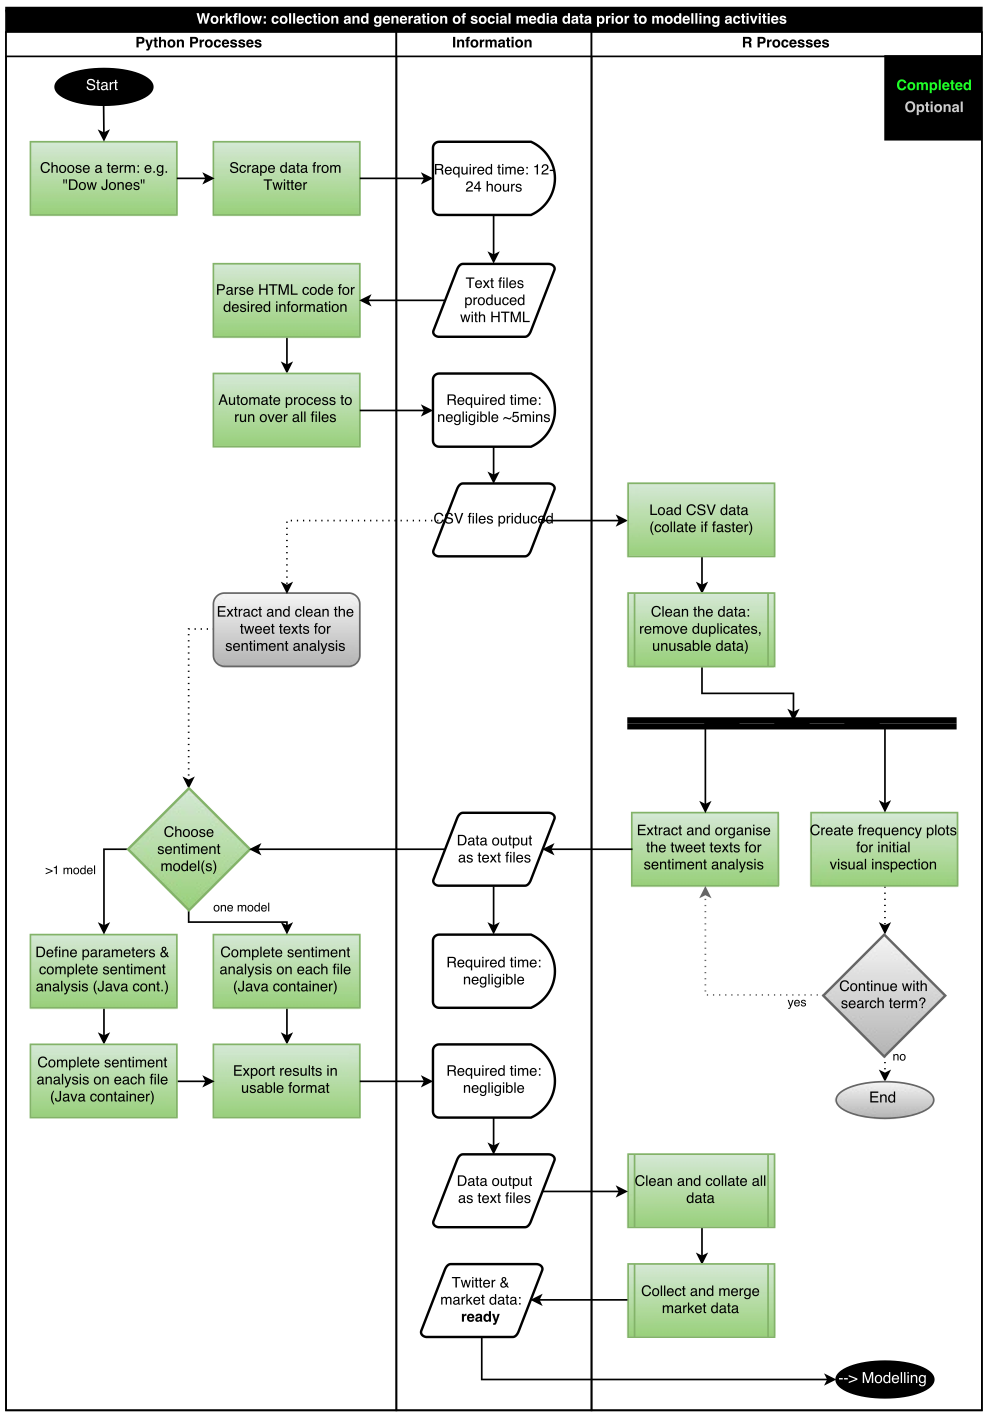
\includegraphics[width=14.5cm]{/Volumes/Mac OS Drive/Thesis/Source Code/Reporting/nwm_Report/images/workflow_scraping.png}


\subsection{Flowchart 2.a - Data preparation \label{flowchart-mod}}
\label{sec-1-2}

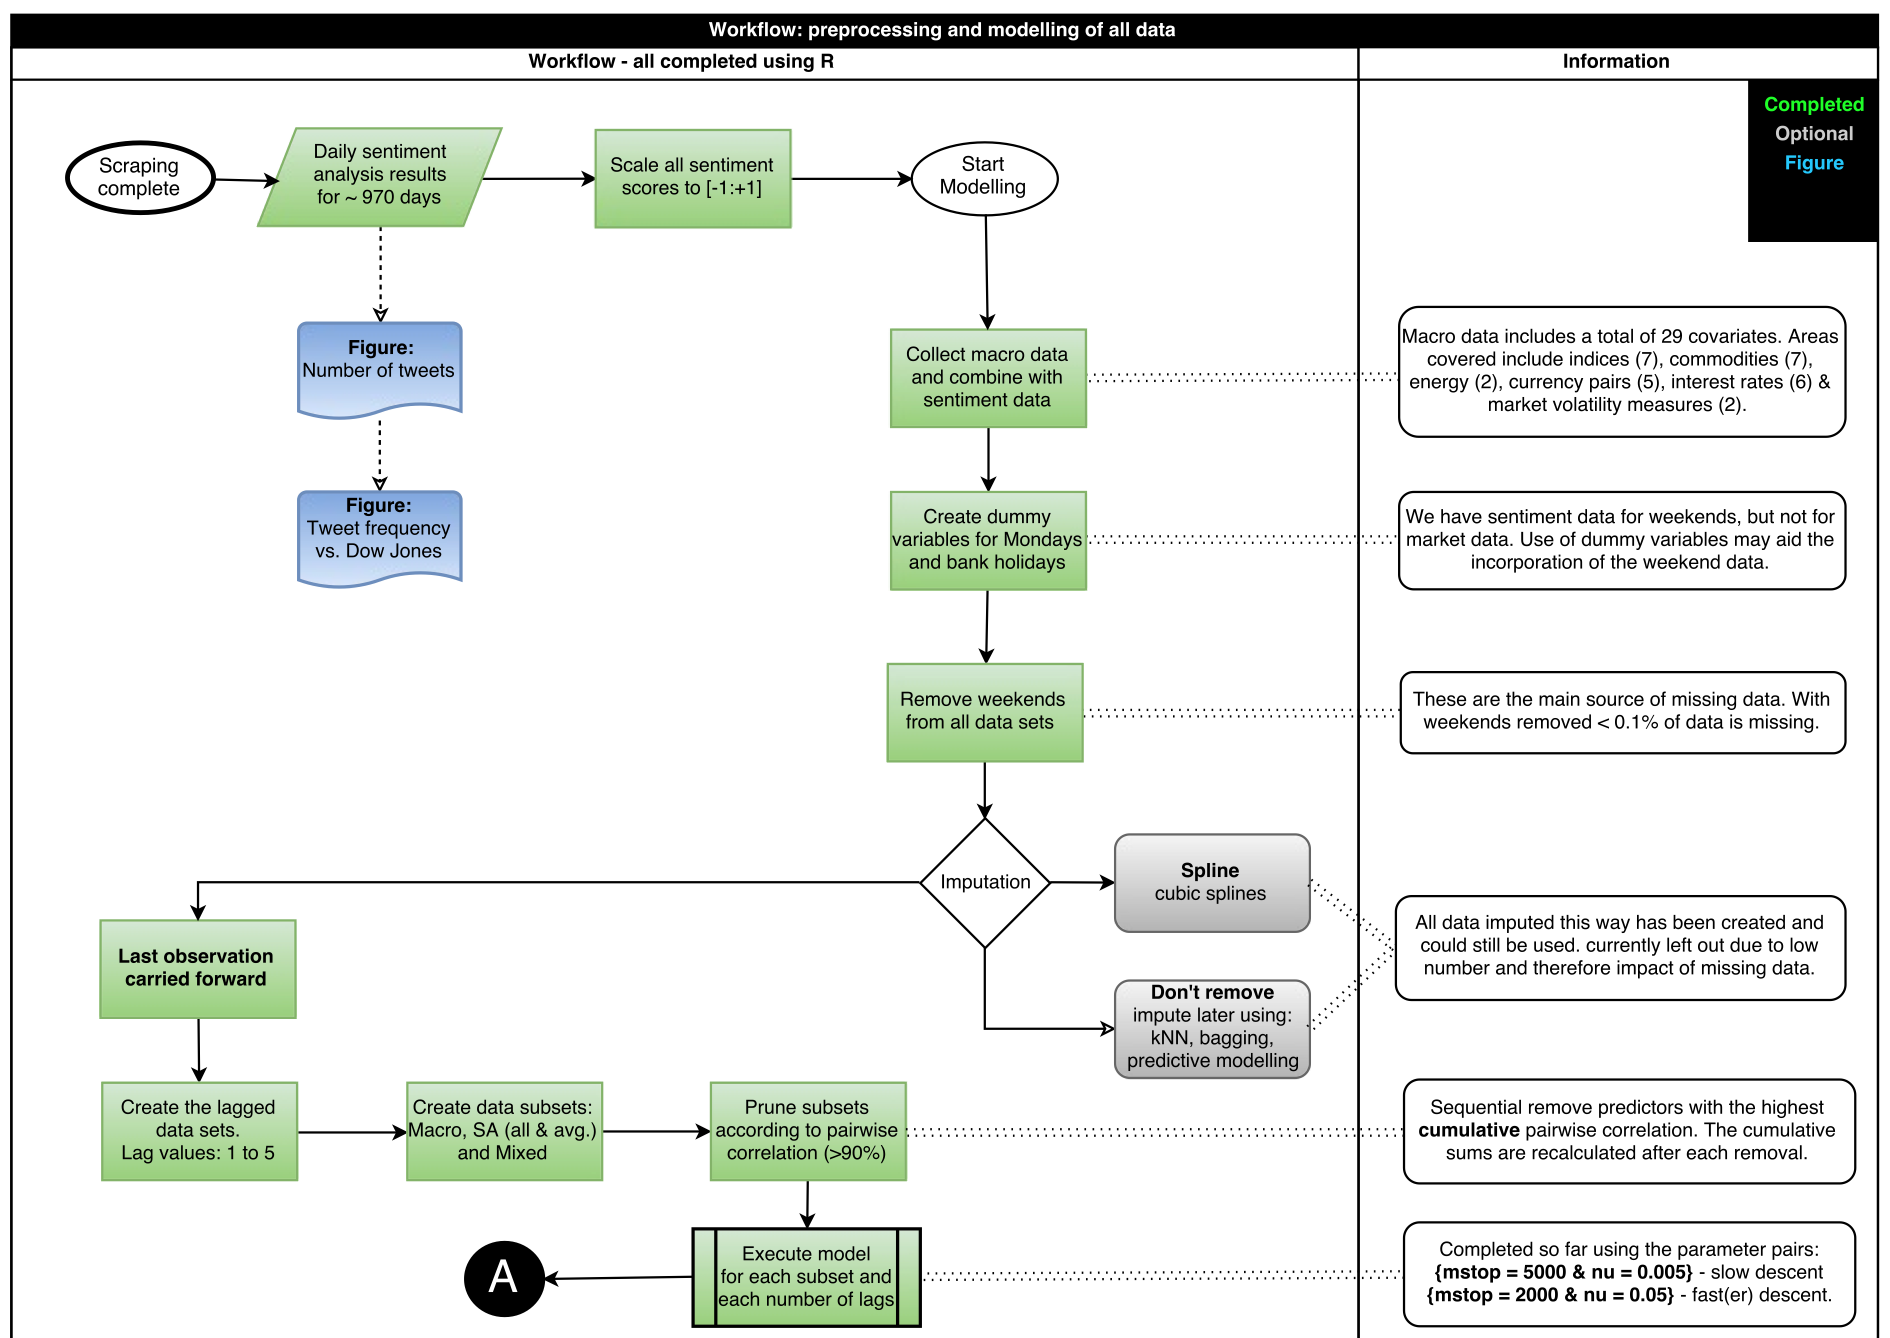
\includegraphics[angle=90,width=15.5cm]{/Volumes/Mac OS Drive/Thesis/Source Code/Reporting/nwm_Report/images/workflow_modelling_1.png}


\subsection{Flowchart 2.b - Modelling}
\label{sec-1-3}
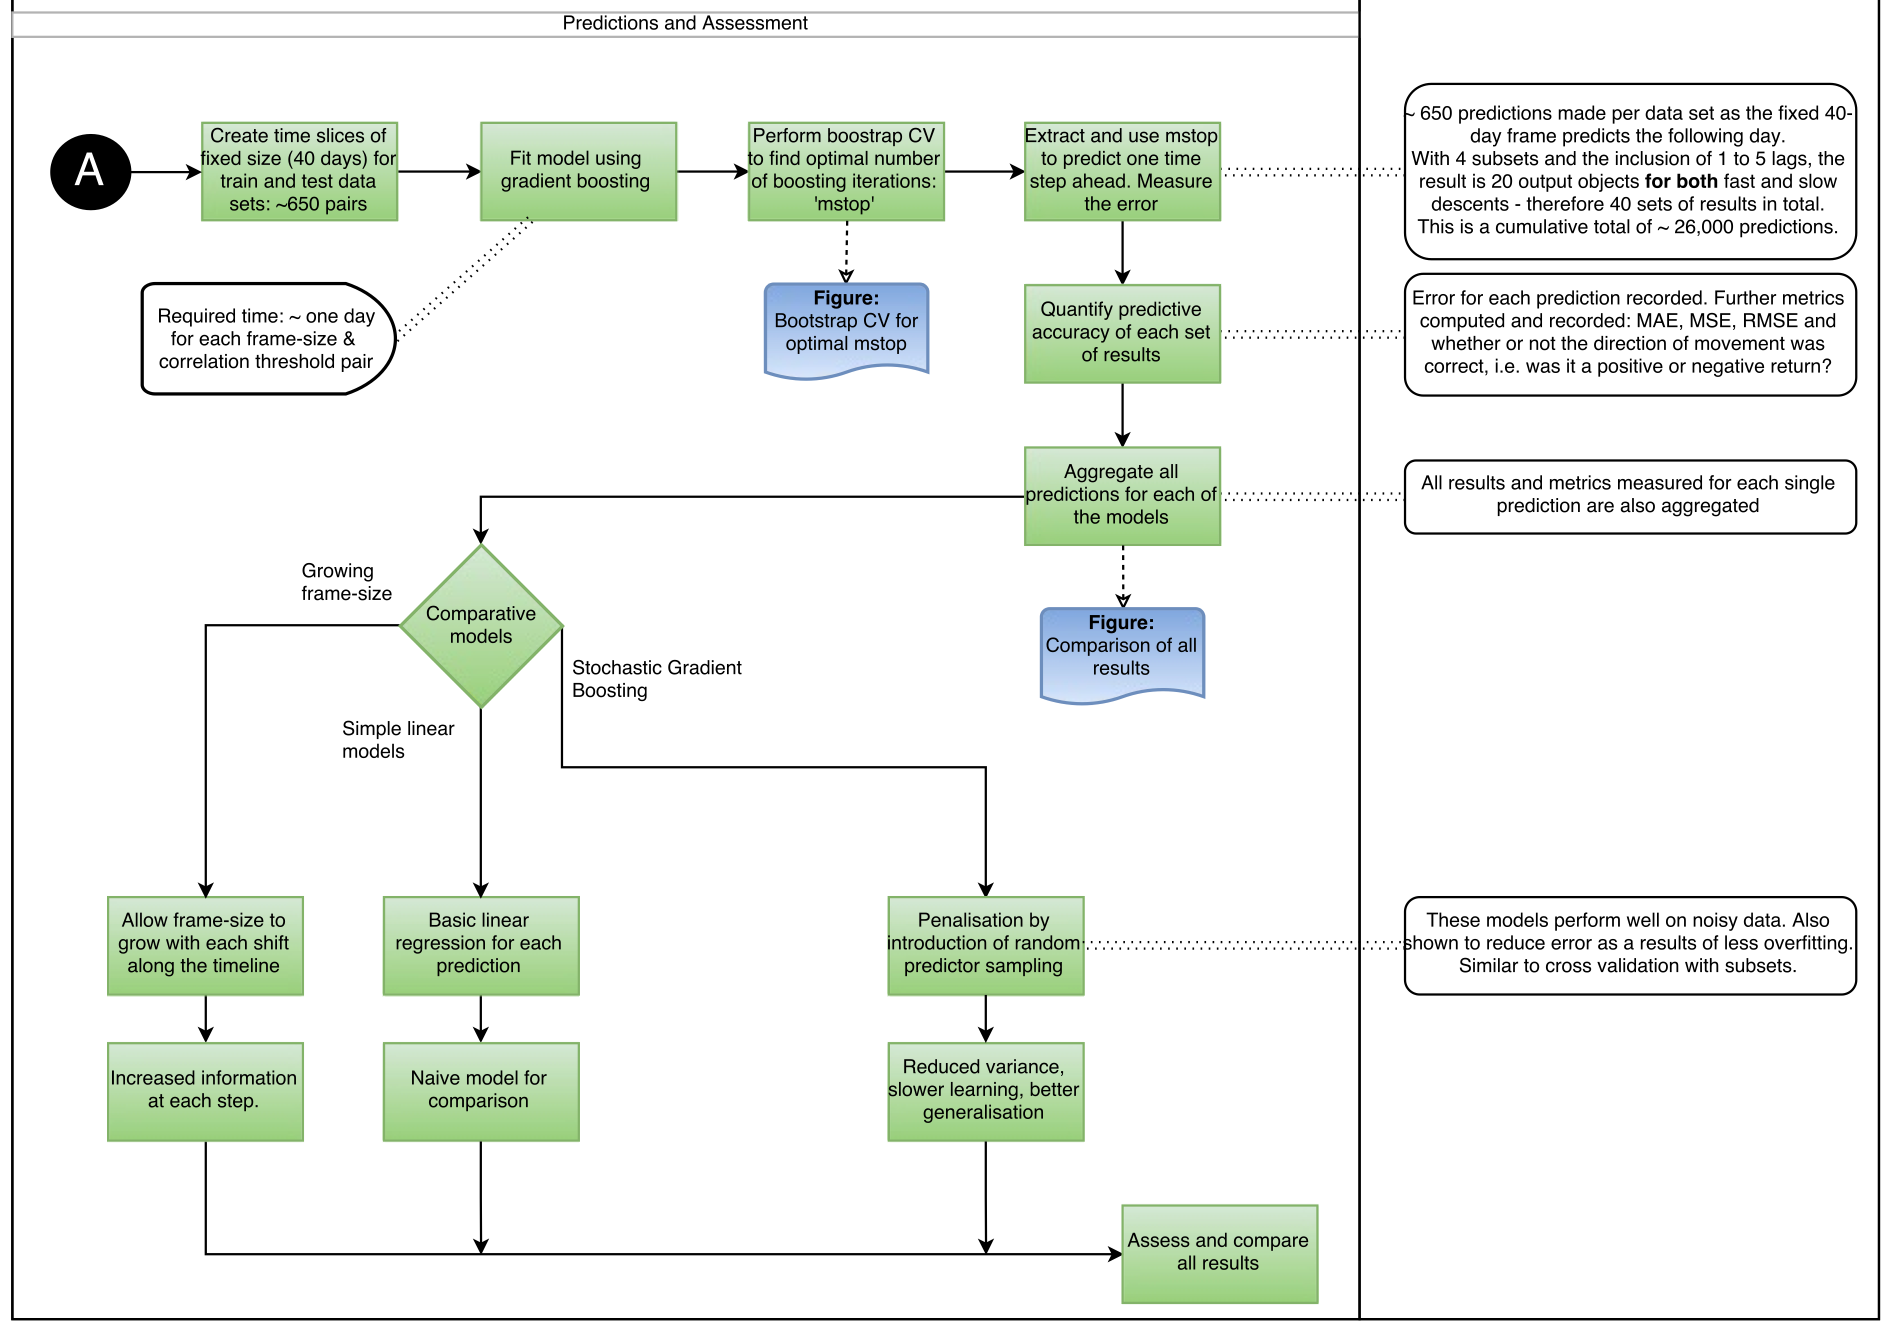
\includegraphics[angle=90,width=15.5cm]{/Volumes/Mac OS Drive/Thesis/Source Code/Reporting/nwm_Report/images/workflow_modelling_2.png}

\pagebreak
% Emacs 24.5.1 (Org mode 8.2.10)
\end{document}